\section{Bluetooth}

Bluetooth è uno standard wireless che permette il collegamento di dispositivi di calcolo, di comunicazione e accessori vari mediante un sistema radio wireless a basso costo, bassa potenza e portata ridotta.
L’unità di base di un sistema Bluetooth è la piconet, composta da un nodo master e da diversi (non più di 7) nodi slave, situati nel raggio di 10 metri. Più piconet possono trovarsi nella stessa stanza e possono essere collegate tramite un nodo ponte, un insieme di piconet è chiamato scatternet.
Tutto si basa sulla comunicazione tra nodo master e nodo slave, il master controlla il clock e decide quale dispositivo può comunicare in ogni intervallo temporale.
I tipi di collegamenti si suddividono in due tipi principali: orientati alla connessione o senza connessione.
Il primo richiede di stabilire una connessione tra i dispositivi prima di inviare i dati, mentre in quello senza connessione il trasmettitore può in qualsiasi momento iniziare a inviare i propri pacchetti purché conosca l’indirizzo del destinatario.
Bluetooth definisce inoltre due tipi di collegamenti a supporto delle applicazioni voce e trasferimento dati: un servizio asincrono senza connessione (ACL) ed un servizio sincrono orientato alla connessione(SCO).
ACL supporta il traffico dati e si basa su un servizio di tipo best-effort (ovvero un servizio che non da alcuna garanzia dell’effettiva consegna dei dati né tantomeno livelli di qualità o priorità garantiti.).
Supporta connessioni a commutazione di pacchetto, connessioni punto-multipunto (multicast) e connessioni simmetriche o asimmetriche.
SCO invece è un collegamento che supporta connessioni con un traffico di tipo real-time e multimediali, prevede connessioni a commutazione di circuito, connessioni punto-punto e connessioni simmetriche.
Bluetooth ha protocolli raggruppati in strati, che non seguono ne modello OSI né TCP/IP.

\section{Si descriva l’algoritmo statico Flooding}

La funzione principale dello strato network è quella d’instradare i pacchetti dal computer sorgente al computer di destinazione.
Lo strato network sfrutta particolari algoritmi detti algoritmi di routing per instradare correttamente i pacchetti nei vari percorsi. Esistono diversi modi di instradare i pacchetti in quanto ci sono molti fattori da tenere in considerazione, però possiamo suddividerli in due grandi tipi: algoritmi non adattivi e algoritmi adattivi.
Gli algoritmi non adattivi basano le loro decisioni su misure e stime del traffico e della topologia corrente, viene calcolato il percorso all’avvio della rete, in modalità fuori linea e viene scaricato nei router, questa procedura si chiama anche routing statico. Gli algoritmi adattivi invece cambiano le loro decisioni secondo le modifiche apportate alla topologia e al traffico.
L’algoritmo di Flooding è un algoritmo statico, in cui ogni pacchetto in arrivo è inviato a tutte le linee tranne quella da cui proviene. I vantaggi che porta si possono elencare in due punti, semplicità di attuazione e assicurazione di ricezione del pacchetto alla stazione desiderata (molteplici volte).
Tuttavia, gli svantaggi sono evidenti, la banda è sprecata, i pacchetti vengono duplicati aumentando la complessità perché vengano scartati, e in caso di cicli i pacchetti potrebbero circolare nella rete all’infinito.
Per questo vanno prese delle precauzioni, una variante un po’ più pratica è chiamata flooding selettivo. In questo algoritmo i router non trasmettono ogni pacchetto verso tutte le linee, ma solo attraverso quelle che vanno approssimativamente nella direzione corretta.
Nella maggior parte delle applicazioni questo algoritmo non è molto utilizzato, salvo casi particolari (i militari lo utilizzano, in quanto un gran numero di router potrebbero saltare in aria, aver questo metodo di trasmissione di pacchetti accerta la ricezione dei dati).
Questo algoritmo viene utilizzato anche come metrica di confronto per altri algoritmi di routing, in quanto sceglie sempre il percorso più breve (scegliendoli tutti LOL), di conseguenza nessun algoritmo può produrre un ritardo più breve (ignorando il tempo di elaborazione dati generato dal processo di flooding).
 
\begin{figure}[H]
\centering
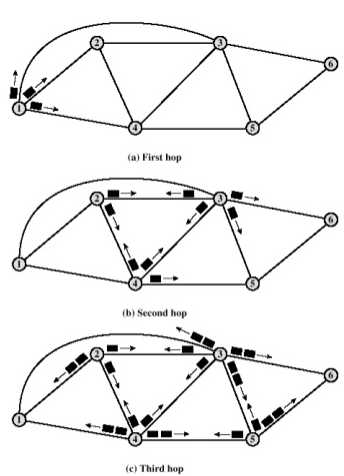
\includegraphics[scale=0.7]{res/img/32_Flooding.png}
%\caption{Didascalia dellimmagine}
\end{figure}

\section{Descrivere il distance vector routing}

La funzione principale dello strato network è quella d’instradare i pacchetti dal computer sorgente al computer di destinazione. Per fare questo vengono utilizzati diversi algoritmi che si possono raggruppare in due grandi gruppo: algoritmi adattivi e non adattivi. Gli algoritmi non adattivi sono anche detti statici, in quanto basano i loro calcoli sulla rete “a freddo” senza tener conto del carico istantaneo o dei problemi di linea, un esempio è l’algoritmo di Flooding.
Generalmente le moderne reti di computer utilizzano algoritmi adattivi, o dinamici se vogliamo. Tra i più popolari ci sono il distance vector routing e il linkstate routing.
Gli algoritmi di routing basati sul vettore delle distanze (distance vector routing) operano facendo in modo che ogni router conservi una tabella (vettore) che definisce la miglior distanza conosciuta per ogni destinazione e la linea che lo conduce ad essa. Queste tabelle vengono aggiornate scambiando informazioni con i router vicini.
Questo algoritmo è basato sull’algoritmo di Bellman-Ford (che calcola i cammini minimi su un grafo (RO insegna)).
Ogni router misura la “distanza” (secondo una metrica che può includere vari fattori) che lo separa dai nodi adiacenti ricevendo i dati dai router vicini. A partire da tali dati, utilizzando l’algoritmo di Bellman-Ford, il router costruisce una tabella che associa ad ogni destinazione conosciuta la stima della distanza che lo separa dalla destinazione e il primo passo del percorso calcolato.
Questo aggiornamento viene fatto periodicamente e dopo sufficienti scambi ciascun router avrà una riga per ogni altro nodo nella rete.
Purtroppo, usando questo algoritmo c’è la possibilità che si creino cicli, e, nel caso in cui un collegamento si interrompe, si può avere una situazione di “count-to-infinity”.
Viene sostituito dal linkstate routing, in quanto l’algoritmo basato sul vettore delle distanze molte volte impiegava troppo tempo a raggiungere la convergenza, e non teneva conto della banda della linea quando sceglieva i percorsi.

\begin{figure}[H]
\centering
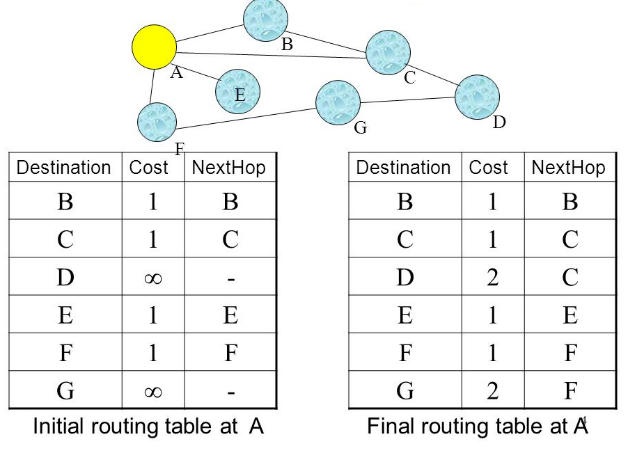
\includegraphics[scale=0.8]{res/img/33_DistanceVectorRouting.png}
%\caption{Didascalia dellimmagine}
\end{figure} 

\section{Descrivere Linkstate routing}

La funzione principale dello strato network è quella d’instradare i pacchetti dal computer sorgente al computer di destinazione. Per fare questo vengono utilizzati diversi algoritmi che si possono raggruppare in due grandi gruppo: algoritmi adattivi e non adattivi. Gli algoritmi non adattivi sono anche detti statici, in quanto basano i loro calcoli sulla rete “a freddo” senza tener conto del carico istantaneo o dei problemi di linea, un esempio è l’algoritmo di Flooding.
Generalmente le moderne reti di computer utilizzano algoritmi adattivi, o dinamici se vogliamo. Tra i più popolari ci sono il distance vector routing e il linkstate routing.
Gli algoritmi di routing basati sullo stato dei collegamenti (linkstate routing) è il sostituto del distance vector routing. L’idea di questo algoritmo si basa su 5 punti:
\begin{itemize}
\item	Scoprire i propri vicini e i relativi indirizzi di rete.
\item	Misurare il ritardo o il costo di ogni vicino.
\item	Costruire un pacchetto che contiene tutte le informazioni raccolte.
\item	Inviare questo pacchetto a tutti gli altri router
\item	Elaborare il percorso più breve verso gli altri router.
\end{itemize}
Un router, prima di tutto, cerca di scoprire chi sono i suoi vicini, lo fa inviando uno speciale pacchetto “HELLO” su ogni linea punto-punto; il router all’altro capo risponde fornendo la propria identità (si noti che i nomi devono essere globalmente unici, in quanto si necessità una non ambiguità durante lo scambio di pacchetti).
Il passo successivo è la misurazione del costo della linea, avviene tramite l’invio di uno speciale pacchetto “ECHO” al quale l’altra parte deve rispondere immediatamente, in base al tempo di andata/ritorno si può ottenere una stima ragionevole del ritardo.
Dopo aver raccolto le informazioni necessarie per lo scambio, ogni router deve costruire un pacchetto contenente tutti i dati. Il pacchetto inizia con l’identità del trasmittente, un numero di sequenza, l’età (contatore che viene decrementato ogni secondo, al raggiungere dello 0 le informazioni provenienti da quel router vengono scartate) e una lista dei vicini. Per ogni vicino è riportato il ritardo misurato. I pacchetti vengono creati periodicamente, oppure in caso di avvenimenti speciali: interruzione della linea o modifica/spegnimento/accensione di un vicino.
La parte più delicata dell’algoritmo è la distribuzione affidabile dei pacchetti che contengono la descrizione dello stato dei collegamenti. Durante la distribuzione e l’installazione, i router che ricevono i primi pacchetti cambieranno i loro percorsi, rischiando di creare inconsistenza, cicli, computer irraggiungibili e cosi via. L’idea fondamentale è quella di utilizzare l’algoritmo di flooding (inviare ogni pacchetto ad ogni linea in uscita (tranne da dov’è arrivato)) un computer che riceve un pacchetto con le informazioni sullo stato della connessione:
\begin{itemize}
\item	Se è duplicato il pacchetto viene scartato
\item	Se è nuovo il pacchetto viene inoltrato a tutte le linee tranne a quella di ricezione (flooding)
\item	Se il numero di sequenza è inferiore al numero più alto visto in quel momento, il pacchetto viene scartato in quanto obsoleto (il router ha informazioni più recenti).
\end{itemize}
Esistono diversi miglioramenti per questo metodo di distribuzione di pacchetti, ma sarebbe troppo lunga da elencare.
Dopo aver accumulato una serie completa di pacchetti sullo stato della connessione, il router può costruire l’intero grafo della sottorete, lo fa utilizzando localmente l’algoritmo di Dijkstra (algoritmo per la costruzione di grafi, simile a quello di Bellman-Ford, non può essere però utilizzato in caso di cammini negativi (RO insegna pt.2)).
Questo algoritmo è molto utilizzato nelle reti reali in quanto può gestire reti composte da molti nodi, converge rapidamente al cammino minimo, difficilmente genera cicli ed è facile da comprendere in quanto ogni nodo ha la mappa completa della rete. Il principale svantaggio è la complessità di realizzazione, anche dovuta alla notevole capacità di memoria ed elaborazione richiesti dai router.
\section{Choke packet}

La funzione principale dello strato network è quella d’instradare i pacchetti dal computer sorgente al computer di destinazione. La decisione del miglior percorso viene effettuato dagli algoritmi di routing (flooding, linkstate o distance vector). Purtroppo, per molteplici motivi, le reti potrebbero congestionarsi, più computer vogliono inviare pacchetti alla stessa destinazione che, non riuscendo ad elaborarli tutti ne perde, questo causa la ritrasmissione che causa ulteriori ingorghi. Questo problema è la congestione ed è un punto critico che va regolamentato.
Il choke packet è uno speciale pacchetto utilizzato per il controllo di flusso in una rete. Un router che rileva una congestione, invia all’host originale del pacchetto che un choke packet per avvertirlo di diminuire il flusso. Quando l’host sorgente riceve il pacchetto speciale diminuisce il flusso (tipicamente lo dimezza) e ignora i successivi choke packet (generalmente ne arrivano in rapida successione), passato un tempo prefissato l’host si rimette all’ascolto, se arrivano altri choke packet in quel frangente diminuisce ulteriormente il flusso, altrimenti riprende gradualmente la velocità normale.
Un problema di questa tecnica è la lentezza di reazione, perché l’host che produce i pacchetti ci mette un certo tempo a ricevere il choke packet e prendere provvedimenti, un miglioramento è dato da hop-by-hop choke packet che diminuisce il flusso per ogni router sul percorso in modo immediato.
 
\begin{figure}[H]
\centering
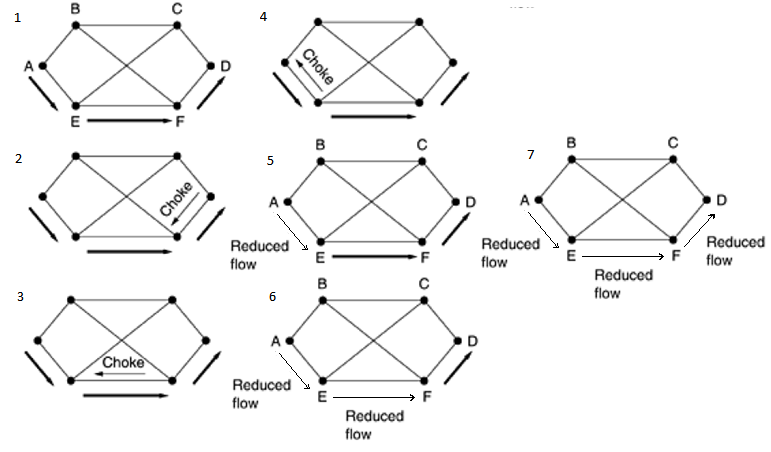
\includegraphics[scale=0.6]{res/img/35_ChokePacket.png}
%\caption{Didascalia dellimmagine}
\end{figure}

\section{Choke packet hop-by-hop}

La funzione principale dello strato network è quella d’instradare i pacchetti dal computer sorgente al computer di destinazione. La decisione del miglior percorso viene effettuato dagli algoritmi di routing (flooding, linkstate o distance vector). Purtroppo, per molteplici motivi, le reti potrebbero congestionarsi, più computer vogliono inviare pacchetti alla stessa destinazione che, non riuscendo ad elaborarli tutti ne perde, questo causa la ritrasmissione che causa ulteriori ingorghi. Questo problema è la congestione ed è un punto critico che va regolamentato.
Il hop-by-hop choke packet è un miglioramento della sua versione precedente (choke packet).
Choke packet aveva il problema di aver un tempo di reazione a prendere provvedimenti troppo lento, il che causava una grossa perdita di dati prima di risolvere il problema
Hop-by-hop choke packet risolve questo problema limitando tutte le stazioni che attraversa in maniera immediata, senza dover attendere di arrivare all’host sorgente.
Questa tecnica rende più veloce il sollievo del router destinatario, ma richiede spazio di buffer nei router “in mezzo” (tra mittente e destinatario).

\begin{figure}[H]
\centering
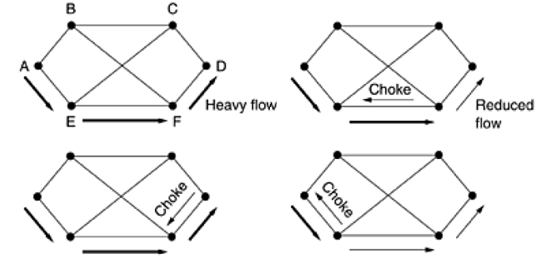
\includegraphics[scale=0.6]{res/img/36_ChokePacketHopbHop.png}
%\caption{Didascalia dellimmagine}
\end{figure}
 
\section{Load shedding}

La funzione principale dello strato network è quella d’instradare i pacchetti dal computer sorgente al computer di destinazione. La decisione del miglior percorso viene effettuato dagli algoritmi di routing (flooding, linkstate o distance vector). Purtroppo, per molteplici motivi, le reti potrebbero congestionarsi, più computer vogliono inviare pacchetti alla stessa destinazione che, non riuscendo ad elaborarli tutti ne perde, questo causa la ritrasmissione che causa ulteriori ingorghi. Questo problema è la congestione ed è un punto critico che va regolamentato.
Quando gli algoritmi di choke packet (puro e hop-by-hop) non bastano per gestire la congestione, i router possono utilizzare la tecnica load shedding che, molto banalmente elimina dei pacchetti casuali in caso di sovraffollamento.
Lo scartare pacchetti casuali non è sempre la scelta migliore, per migliorare l’algoritmo infatti la scelta può basarsi sull’applicazione in esecuzione, esistono due criteri generali per identificare queste scelte, wine e milk.
Wine da più importanza ai pacchetti vecchi, scarta di conseguenza quelli nuovi (vecchio è meglio del nuovo), milk invece al contrario da importanza maggiore ai pacchetti nuovi (nuovo è migliore del vecchio).
Questa tecnica permette numerose applicazioni e metodi per implementarla (oltre a wine e milk) questo permette di tenere sotto controllo possibili momenti di congestione.

\section{Red (Random Early Detection)}

Nello strato network esistono numerosi algoritmi di instradamento per portare un pacchetto da una destinazione ad un mittente (flooding, distance vector, linkstate), quando questa linea si congestiona esistono algoritmi che permettono di gestire la congestione e risolvere il problema (choke packet e load shedding). Risulta tuttavia più semplice gestire la congestione appena viene rilevata, non cercare di porvi rimedio dopo averle dato il tempo di bloccare tutta la linea.
Questa osservazione conduce all’idea di scartare i pacchetti prima che il buffer sia completamente pieno, da qui nasce un celebre algoritmo usato per mettere in pratica questo schema: RED (Random Early Detection).
Red in pratica fa in modo che i router scartino i pacchetti prima che la situazione diventi senza speranza (early). Per stabilire quando è il momento giusto per iniziare a scartare i pacchetti, i router mantengono una media mobile delle lunghezze delle code. Quando la lunghezza media su una linea supera una soglia di guardia allora quella determinata linea è considerata congestionata e prende le dovute azioni di correzione. Il massimo che può fare purtroppo è scegliere un pacchetto a caso dalla coda che ha attivato “l’azione difensiva”. Per segnalare il rischio di congestione il router potrebbe inviare un choke packet per chiedere la diminuzione di flusso, tuttavia questo congestionerebbe ulteriormente le linee. La strategia migliore è scartare banalmente il pacchetto e attendere che la sorgente lo re-invii a causa del mancato acknowledgement. Questa ultima strategia funziona solo quando le sorgenti rispondono ai pacchetti perduti rallentando il flusso. Nelle reti wireless, dove la maggior parte dei pacchetti persi è a causa del rumore, questo non avviene, è infatti impossibile usarla in quei casi.

\section{Reverse Path Forwarding}

I router spesso necessitano di inviare messaggi a molti o a tutti gli altri host. Questi tipi di trasmissioni sono dette trasmissioni broadcast.
L’algoritmo di routing più quotato per questo genere di trasmissioni è sicuramente quello di flooding, in quanto invia i pacchetti a tutte le stazioni vicine (tranne quella da cui ha ricevuto il pacchetto). Un problema di questa tecnica è sicuramente lo spreco di banda e la creazione di troppi pacchetti.
Per ovviare a questo problema sono stati creati numerosi algoritmi che cercano di migliorare questo sistema di broadcasting.
Con il Reverse path forwarding il router che riceve un pacchetto controlla se gli è giunto da una linea che normalmente è utilizzata per inviare i pacchetti alla sorgente (ovvero che sia la linea con cammino minimo da lui alla sorgente). In caso affermativo, c’è una forte probabilità che il pacchetto broadcast abbia seguito il percorso migliore dalla sorgente fino a lui, di conseguenza lo copia e lo inoltra a tutte le linee (tranne quella da cui l’ha ricevuto). Se invece il pacchetto broadcast è giunto attraverso una linea diversa dalla preferita per raggiungere la sorgente, il pacchetto viene scartato in quanto è probabile si tratti di un duplicato.
Questo algoritmo previene il problema dell’IP spoofing (falsificazione dell’indirizzo del mittente).
La sua implementazione è efficiente e non richiede di conoscere la mappa della sottorete, liste di destinazione o mappe di bit per ogni pacchetto broadcast, il che lo rende anche di facile implementazione.

\section{Quality of Service (QoS)}

Un flusso di pacchetti da una sorgente a una destinazione è chiamato, appunto, flusso.
Ogni flusso viene regolamentato per il percorso da effettuare e quando effettuarlo, i metodi di gestione della congestione e così via.
Ogni flusso ha le sue esigenze, in base all’applicazione che sta servendo, possiamo quindi caratterizzare queste esigenze in quattro parametri primari: affidabilità, ritardo, jitter e banda. Insieme, questi parametri determinano la QoS (Quality of Service), ossia la qualità del servizio richiesta dal flusso.
\begin{itemize}
\item	Affidabilità: nessun bit può essere trasmesso in modo scorretto. Questo obiettivo viene di solito raggiunto creando il checksum di ogni pacchetto e verificandolo alla destinazione. Questo parametro è ricercato da applicazioni tipo la posta elettronica o trasferimento di file, che necessitano di un’alta affidabilità, applicazioni come audio o video possono tollerare errori, perciò non viene elaborato o verificato nessun checksum.
\item	Ritardo: il ritardo dei pacchetti in applicazioni come la posta elettronica o il trasferimento file non è molto sentito, è importante invece in applicazioni come telefonate o videoconferenze.
\item	Jitter: Il Jitter non è altro che la variazione del segnale in modo casuale. Questo può portare ad una ricezione di dati in intervalli irregolari, applicazioni come può essere la posta elettronica o il trasferimento file non sono molto soggette a questo problema. Lo sono invece per applicazioni di login remoto o di streaming video, a causa della variazione casuale della trasmissione, il risultato è terribile.
\item	Banda: ogni applicazione differisce per l’esigenza di banda, posta elettronica e accesso remoto non ne richiede molta, il video in tutte le sue forme invece sì.
\end{itemize}
Nessuna tecnica è in grado di fornire QoS efficiente e sicura in modo ottimo. 

\begin{figure}[H]
\centering
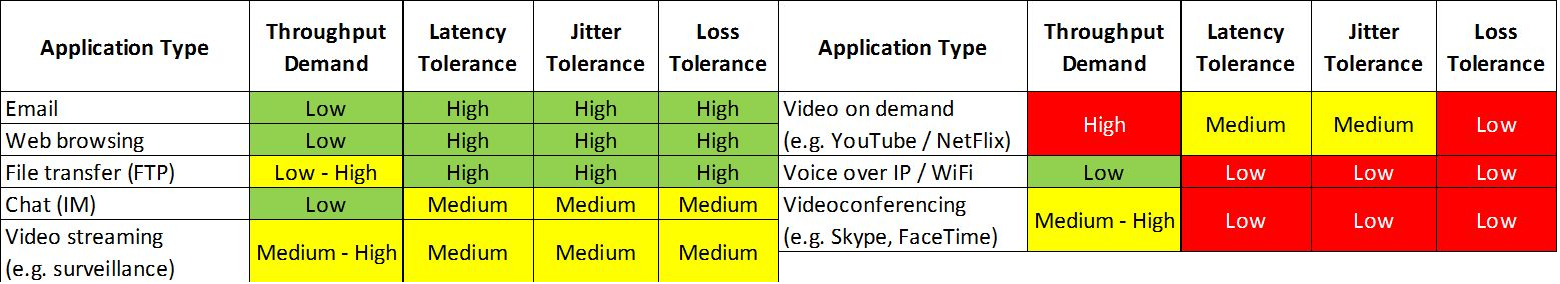
\includegraphics[scale=0.3]{res/img/40_QoS.png}
%\caption{Didascalia dellimmagine}
\end{figure}
